%%% Hlavní soubor. Zde se definují základní parametry a odkazuje se na ostatní části. %%%

%% Verze pro jednostranný tisk:
% Okraje: levý 40mm, pravý 25mm, horní a dolní 25mm
% (ale pozor, LaTeX si sám přidává 1in)
\documentclass[12pt,a4paper]{report}
\setlength\textwidth{145mm}
\setlength\textheight{247mm}
\setlength\oddsidemargin{15mm}
\setlength\evensidemargin{15mm}
\setlength\topmargin{0mm}
\setlength\headsep{0mm}
\setlength\headheight{0mm}
% \openright zařídí, aby následující text začínal na pravé straně knihy
\let\openright=\clearpage

%% Pokud tiskneme oboustranně:
% \documentclass[12pt,a4paper,twoside,openright]{report}
% \setlength\textwidth{145mm}
% \setlength\textheight{247mm}
% \setlength\oddsidemargin{14.2mm}
% \setlength\evensidemargin{0mm}
% \setlength\topmargin{0mm}
% \setlength\headsep{0mm}
% \setlength\headheight{0mm}
% \let\openright=\cleardoublepage

%% Vytváříme PDF/A-2u
\usepackage[a-2u]{pdfx}

%% Přepneme na českou sazbu a fonty Latin Modern
\usepackage[czech]{babel}
\usepackage{lmodern}
\usepackage[T1]{fontenc}
\usepackage{textcomp}

%% Použité kódování znaků: obvykle latin2, cp1250 nebo utf8:
\usepackage[utf8]{inputenc}

%%% Další užitečné balíčky (jsou součástí běžných distribucí LaTeXu)
\usepackage{amsmath}        % rozšíření pro sazbu matematiky
\usepackage{amsfonts}       % matematické fonty
\usepackage{amsthm}         % sazba vět, definic apod.
\usepackage{bbding}         % balíček s nejrůznějšími symboly
			    % (čtverečky, hvězdičky, tužtičky, nůžtičky, ...)
\usepackage{bm}             % tučné symboly (příkaz \bm)
\usepackage{graphicx}       % vkládání obrázků
\usepackage{fancyvrb}       % vylepšené prostředí pro strojové písmo
\usepackage{indentfirst}    % zavede odsazení 1. odstavce kapitoly
\usepackage{natbib}         % zajištuje možnost odkazovat na literaturu
			    % stylem AUTOR (ROK), resp. AUTOR [ČÍSLO]
\usepackage[nottoc]{tocbibind} % zajistí přidání seznamu literatury,
                            % obrázků a tabulek do obsahu
\usepackage{icomma}         % inteligetní čárka v matematickém módu
\usepackage{dcolumn}        % lepší zarovnání sloupců v tabulkách
\usepackage{booktabs}       % lepší vodorovné linky v tabulkách
\usepackage{paralist}       % lepší enumerate a itemize
\usepackage{xcolor}         % barevná sazba

%%% Údaje o práci

% Název práce v jazyce práce (přesně podle zadání)
\def\NazevPrace{Vizuální browser grafových dat}

% Název práce v angličtině
\def\NazevPraceEN{Visual browser of graph data}

% Jméno autora
\def\AutorPrace{Štěpán Stenchlák}

% Rok odevzdání
\def\RokOdevzdani{2020}

% Název katedry nebo ústavu, kde byla práce oficiálně zadána
% (dle Organizační struktury MFF UK, případně plný název pracoviště mimo MFF)
\def\Katedra{Katedra softwarového inženýrství}
\def\KatedraEN{Name of the department}

% Jedná se o katedru (department) nebo o ústav (institute)?
\def\TypPracoviste{Katedra}
\def\TypPracovisteEN{Department}

% Vedoucí práce: Jméno a příjmení s~tituly
\def\Vedouci{doc. Mgr. Martin Nečaský, Ph.D.}

% Pracoviště vedoucího (opět dle Organizační struktury MFF)
\def\KatedraVedouciho{katedra}
\def\KatedraVedoucihoEN{department}

% Studijní program a obor
\def\StudijniProgram{Informatika}
\def\StudijniObor{Softwarové a datové inženýrství}

% Nepovinné poděkování (vedoucímu práce, konzultantovi, tomu, kdo
% zapůjčil software, literaturu apod.)
\def\Podekovani{%
Poděkování.
}

% Abstrakt (doporučený rozsah cca 80-200 slov; nejedná se o zadání práce)
\def\Abstrakt{%
Abstrakt.
}
\def\AbstraktEN{%
Abstract.
}

% 3 až 5 klíčových slov (doporučeno), každé uzavřeno ve složených závorkách
\def\KlicovaSlova{%
{klíčová} {slova}
}
\def\KlicovaSlovaEN{%
{key} {words}
}

%% Balíček hyperref, kterým jdou vyrábět klikací odkazy v PDF,
%% ale hlavně ho používáme k uložení metadat do PDF (včetně obsahu).
%% Většinu nastavítek přednastaví balíček pdfx.
\hypersetup{unicode}
\hypersetup{breaklinks=true}

%% Definice různých užitečných maker (viz popis uvnitř souboru)
%%% Tento soubor obsahuje definice různých užitečných maker a prostředí %%%
%%% Další makra připisujte sem, ať nepřekáží v ostatních souborech.     %%%

%%% Drobné úpravy stylu

% Tato makra přesvědčují mírně ošklivým trikem LaTeX, aby hlavičky kapitol
% sázel příčetněji a nevynechával nad nimi spoustu místa. Směle ignorujte.
\makeatletter
\def\@makechapterhead#1{
  {\parindent \z@ \raggedright \normalfont
   \Huge\bfseries \thechapter. #1
   \par\nobreak
   \vskip 20\p@
}}
\def\@makeschapterhead#1{
  {\parindent \z@ \raggedright \normalfont
   \Huge\bfseries #1
   \par\nobreak
   \vskip 20\p@
}}
\makeatother

% Toto makro definuje kapitolu, která není očíslovaná, ale je uvedena v obsahu.
\def\chapwithtoc#1{
\chapter*{#1}
\addcontentsline{toc}{chapter}{#1}
}

% Trochu volnější nastavení dělení slov, než je default.
\lefthyphenmin=2
\righthyphenmin=2

% Zapne černé "slimáky" na koncích řádků, které přetekly, abychom si
% jich lépe všimli.
\overfullrule=1mm

%%% Makra pro definice, věty, tvrzení, příklady, ... (vyžaduje baliček amsthm)

\theoremstyle{plain}
\newtheorem{veta}{Věta}
\newtheorem{lemma}[veta]{Lemma}
\newtheorem{tvrz}[veta]{Tvrzení}

\theoremstyle{plain}
\newtheorem{definice}{Definice}

\theoremstyle{definition}
\newtheorem*{dusl}{Důsledek}
\newtheorem*{pozn}{Poznámka}
\newtheorem*{prikl}{Příklad}

%%% Prostředí pro důkazy

\newenvironment{dukaz}{
  \par\medskip\noindent
  \textit{Důkaz}.
}{
\newline
\rightline{$\qedsymbol$}
}

%%% Prostředí pro sazbu kódu, případně vstupu/výstupu počítačových
%%% programů. (Vyžaduje balíček fancyvrb -- fancy verbatim.)

\DefineVerbatimEnvironment{code}{Verbatim}{fontsize=\small, frame=single}

%%% Prostor reálných, resp. přirozených čísel
\newcommand{\R}{\mathbb{R}}
\newcommand{\N}{\mathbb{N}}

%%% Užitečné operátory pro statistiku a pravděpodobnost
\DeclareMathOperator{\pr}{\textsf{P}}
\DeclareMathOperator{\E}{\textsf{E}\,}
\DeclareMathOperator{\var}{\textrm{var}}
\DeclareMathOperator{\sd}{\textrm{sd}}

%%% Příkaz pro transpozici vektoru/matice
\newcommand{\T}[1]{#1^\top}

%%% Vychytávky pro matematiku
\newcommand{\goto}{\rightarrow}
\newcommand{\gotop}{\stackrel{P}{\longrightarrow}}
\newcommand{\maon}[1]{o(n^{#1})}
\newcommand{\abs}[1]{\left|{#1}\right|}
\newcommand{\dint}{\int_0^\tau\!\!\int_0^\tau}
\newcommand{\isqr}[1]{\frac{1}{\sqrt{#1}}}

%%% Vychytávky pro tabulky
\newcommand{\pulrad}[1]{\raisebox{1.5ex}[0pt]{#1}}
\newcommand{\mc}[1]{\multicolumn{1}{c}{#1}}


%% Titulní strana a různé povinné informační strany
\begin{document}
%%% Titulní strana práce a další povinné informační strany

%%% Titulní strana práce

\pagestyle{empty}
\hypersetup{pageanchor=false}

\begin{center}

\centerline{\mbox{
\includegraphics[width=166mm]{img/logo-cs.pdf}}}

\vspace{-8mm}
\vfill

{\bf\Large BAKALÁŘSKÁ PRÁCE}

\vfill

{\LARGE\AutorPrace}

\vspace{15mm}

{\LARGE\bfseries\NazevPrace}

\vfill

\Katedra

\vfill

{
\centerline{\vbox{\halign{\hbox to 0.45\hsize{\hfil #}&\hskip 0.5em\parbox[t]{0.45\hsize}{\raggedright #}\cr
Vedoucí bakalářské práce:&\Vedouci \cr
\noalign{\vspace{2mm}}
Studijní program:&\StudijniProgram \cr
\noalign{\vspace{2mm}}
Studijní obor:&\StudijniObor \cr
}}}}

\vfill

% Zde doplňte rok
Praha \RokOdevzdani

\end{center}

\newpage

%%% Následuje vevázaný list -- kopie podepsaného "Zadání bakalářské práce".
%%% Toto zadání NENÍ součástí elektronické verze práce, nescanovat.

%%% Strana s čestným prohlášením k bakalářské práci

\openright
\hypersetup{pageanchor=true}
\pagestyle{plain}
\pagenumbering{roman}
\vglue 0pt plus 1fill

\noindent
Prohlašuji, že jsem tuto bakalářskou práci vypracoval(a) samostatně a výhradně
s~použitím citovaných pramenů, literatury a dalších odborných zdrojů.
Tato práce nebyla využita k získání jiného nebo stejného titulu.

\medskip\noindent
Beru na~vědomí, že se na moji práci vztahují práva a povinnosti vyplývající
ze zákona č. 121/2000 Sb., autorského zákona v~platném znění, zejména skutečnost,
že Univerzita Karlova má právo na~uzavření licenční smlouvy o~užití této
práce jako školního díla podle §60 odst. 1 autorského zákona.

\vspace{10mm}

\hbox{\hbox to 0.5\hsize{%
V \hbox to 6em{\dotfill} dne \hbox to 6em{\dotfill}
\hss}\hbox to 0.5\hsize{\dotfill\quad}}
\smallskip
\hbox{\hbox to 0.5\hsize{}\hbox to 0.5\hsize{\hfil Podpis autora\hfil}}

\vspace{20mm}
\newpage

%%% Poděkování

\openright

\noindent
\Podekovani

\newpage

%%% Povinná informační strana bakalářské práce

\openright

\vbox to 0.5\vsize{
\setlength\parindent{0mm}
\setlength\parskip{5mm}

Název práce:
\NazevPrace

Autor:
\AutorPrace

\TypPracoviste:
\Katedra

Vedoucí bakalářské práce:
\Vedouci, \KatedraVedouciho

Abstrakt:
\Abstrakt

Klíčová slova:
\KlicovaSlova

\vss}\nobreak\vbox to 0.49\vsize{
\setlength\parindent{0mm}
\setlength\parskip{5mm}

Title:
\NazevPraceEN

Author:
\AutorPrace

\TypPracovisteEN:
\KatedraEN

Supervisor:
\Vedouci, \KatedraVedoucihoEN

Abstract:
\AbstraktEN

Keywords:
\KlicovaSlovaEN

\vss}

\newpage

\openright
\pagestyle{plain}
\pagenumbering{arabic}
\setcounter{page}{1}


%%% Strana s automaticky generovaným obsahem bakalářské práce

\tableofcontents

%%% Jednotlivé kapitoly práce jsou pro přehlednost uloženy v samostatných souborech
\chapter*{Úvod}
\addcontentsline{toc}{chapter}{Úvod}

Na internetu je dnes možné najít téměř cokoli, kupříkladu stav počasí, encyklopedické informace, odborné publikace, jízdní řády a podobně. Tyto informace jsou uloženy jako webové stránky systému WWW (World Wide Web) a kterýkoli uživatel internetu má k nim přístup a může z nich čerpat.

Pro lidi je systém WWW vyhovující zdroj informací, nicméně narazíme na problém, pokud chceme tyto informace číst strojově. WWW totiž nepopisuje, jak by měly být informace na internetu prezentovány. Každý publikovatel si může data zveřejnit jinak, například tabulkou, odrážkovým seznamem, nebo ve větách. Tyto informace jsou stále snadno čitelné pro člověka, ale obtížně čitelné pro stroj.

Možností řešení tohoto problému je zveřejňovat data i ve strojové podobně. Nabízí se například tabulky ve formátu CSV, nebo komplikovanější data ve formátu JSON a XML. Zde je již snadné číst data a dál je zpracovávat, ale programátor je stále nucen pochopit a přizpůsobit program na rozhraní těchto dat.

Možným řešením se nabízí popsat data pomocí RDF frameworku, jež je důkladněji rozebrán v následující kapitole.

\bigskip

Tato práce se zabývá reprezentací dat popsaných právě pomocí RDF. RDF reprezentuje entity z reálného světa jako vrcholy grafu a jejich vlastnosti pomocí hran propojující tyto entity. Data uložená v grafových databázích jsou snadno čitelná počítačovými programy a je jednoduché propojovat různé datové zdroje do větších celků a provádět nad nimi dotazy.

Jako veškerá strojová data je potřeba i tyto grafová data vizualizovat. Příkladem může být datový analytik, který se chce přesvědčit, že jsou data uložena tak, jak bylo zamýšleno.

Jako modelový příklad vizualizace uveďme entitu Karla Čapka a některá jeho data, jež má o něm uložená Wikipedie.

\begin{figure}[h]
    \centering
    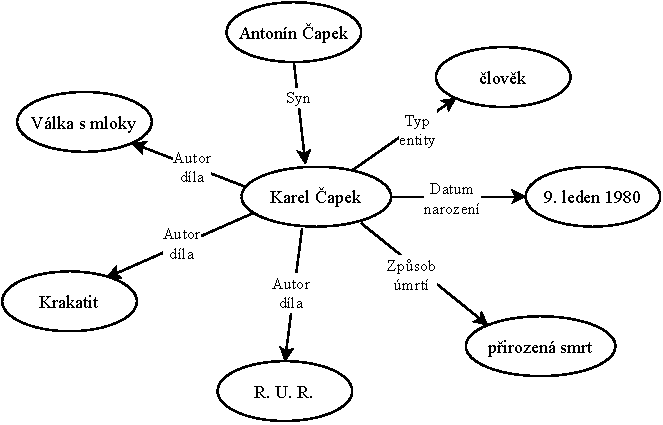
\includegraphics{media/capek-full.pdf}
    \caption{Ukázka části grafu jež může reprezentovat Karla Čapka.}
    \label{fig:capek-full}
\end{figure}

Jak vidíme z obrázku \ref{fig:capek-full}, zobrazit všechna data k vrcholu může být velmi nepřehledné a takovýchto vrcholů může být stovky. Pokud nás například zajímají pouze díla Karla Čapka, určitě v grafu nebudeme chtít mít informaci, že je Karel Čapek člověk. Tuto situaci můžeme vyřešit tak, že se na entity grafu budeme dívat pouze určitým pohledem a tedy zobrazíme pouze ty vztahy k vrcholu, jež odpovídají danému pohledu.

Kupříkladu pokud bychom chtěli procházet rodokmenem, je vhodné se na Karla Čapka dívat jako na osobu, jež má rodiče a sama může být rodičem ostatních osob. V tuto chvíli nás nezajímají ostatní vlastnosti jako knihy, které napsal, nebo ocenění, která získal. Na Karla Čapka se ale můžeme dívat i jako na spisovatele, kde nás pak zajímají pouze jeho díla a rodinné vztahy můžeme skrýt. Příklad takovýchto pohledů je na obrázku \ref{fig:capek-part}.

\begin{figure}[h]
    \centering
    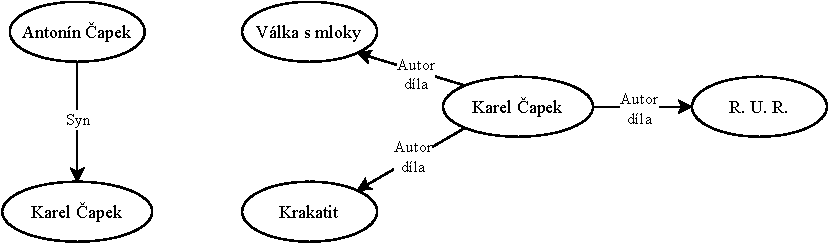
\includegraphics{media/capek-part.pdf}
    \caption{Pohled na Karla Čapka jako na osobu mající rodinu (vlevo) a na spisovatele jež je autorem literárních děl (vpravo)}
    \label{fig:capek-part}
\end{figure}

Tento způsob procházení grafových dat sice vyžaduje předem nadefinovat pohledy, ale procházení dat je pak jednoduché a velmi přehledné.

\section{Cíl práce}

Cílem této práce je vyrobit webovou aplikaci, jež by na základě předem definovaných pohledů vizualizovala grafová data a umožňovala uživateli procházet tento graf a objevovat nové vrcholy. Protože je žádoucí mít více pohledů na konkrétní typ vrcholu, pohledy jsou seskupeny do takzvaných konfigurací. Konfigurace pak popisuje nejen pohledy na různé typy vrcholů, ale i jaké vrcholy lze takto vizualizovat a z jakých zdrojů čerpat.

Konfigurace, jež jsou použité v aplikaci jsou například:
\begin{itemize}
    \item \textbf{Procházení živočichů na Wikidatech} - Uživatel může vizualizovat jednotlivé rostlinné a živočišné druhy a procházet je podle rozdělení do taxonů.
    \item \textbf{Procházení slavných osobností na Wikidatech} - Uživatel může procházet slavné osobnosti a nechat si načíst jejich filmová a literární díla a rodinné vztahy.
\end{itemize}

Motivací pro tuto práci je i výzkum\footnote{\citet{Klimek2019}} z roku 2019, jež dochází k závěru, že vizualizační nástroje, které by vyžadovaly malou znalost uživatele týkající se technických detailů RDF, chybí. Tato práce si klade za cíl odstínit běžného uživatele od těchto technických detailů, avšak bude obsahovat možnosti i pro technicky zdatnější uživatele, jež RDF rozumí.

%%% Fiktivní kapitola s ukázkami sazby

\chapter{Vue.js framework}
Klientská část aplikace je postavena nad Vue.js frameworkem, jež je populární JavaScriptový framework na stavbu uživatelských rozhraní. Protože některé z jeho funkcionalit byly použity v klíčových částech aplikace, je nutné čtenáře obeznámit alespoň se základním principem fungování frameworku.

\section{Vuex}
Vue.js framework, podobně jako konkurenční React\footnote{\url{https://reactjs.org/}} (Facebook) nebo Angular\footnote{\url{https://angularjs.org/}} (Google), využívají principu sledování stavu aplikace (jejich dat) pro automatickou změnu DOMu webové stránky. V praxi to znamená, že programátor může velice snadno napsat kód, který generuje uživatelské rozhraní na základě dat, která mohou být libovolně měněna bez nutnosti řešit problém, zda ke změně vůbec došlo a které části aplikace mají být o změně stavu informovány. Ve Vue tuto funkcionalitu zastává právě Vuex\footnote{\url{https://vuex.vuejs.org/}}, jež je možný používat samostatně.

Vuex drží stav aplikace jako jeden objekt (tedy slouží jako centrální úložiště dat pro celou aplikaci). Tento objekt se nazývá \textbf{store}. Změny ve storu mohou být sledovány Vuexem pro vykonání libovolných akcí, například překreslení textu na stránce, jež byl vykreslen Vue frameworkem.

\newcommand{\inlinecode}{\texttt}

Vrátíme-li se k původnímu příkladu, programátorovi stačí přiřadit do proměnné, jež je spravovaná Vuexem, novou hodnotu a Vuex se postará o zavolání všech komponent, které tuto proměnnou využívají a tyto komponenty na stránce překreslí původní hodnotu na novou. Překreslení přitom proběhne až poté, co skončí průběh aktuální funkce. Tohoto je docíleno pomocí \\ \texttt{Window.requestAnimationFrame()}. Díky tomuto můžeme stav v rámci průběhu jedné funkce modifikovat vícekrát se skoro nulovým dopadem na celkový výkon aplikace.

\subsection{Computed properties}

Kromě této funkcionality Vuex nabízí takzvané \textbf{gettery}, jež jsou ve Vue frameworku nazývány jako \textbf{computed properties}. Jedná se o funkce, které využívají data ze storu pro výpočet dat nových. Výhoda takovýchto getterů je ta, že Vuex dokáže výsledky těchto funkcí cachovat a přepočítává je pouze tehdy, změní-li se data původní. Interně gettery fungují tak, že při zavolání klientské funkce Vuex sleduje které části storu byly dotázany a ty pak sleduje na změnu jež invaliduje cache konkrétního getteru. Při příštím požadavku na hodnotu se pak klientská funkce volá znovu a celá operace se opakuje.

Tyto computed properties jsou v aplikaci využívány často. Kupříkladu funkce, která počítá, zda je sousední uzel vybrán. Na takovouto hodnotu se v aplikaci mohu ptát libovolně krát, ale počítá se pouze tehdy, když se množina sousedních uzlů vrcholu změní, nebo se změní právě označení uzlu z množiny.

\subsection{Watchers}

Ve Vue lze využívat i \textbf{watch}ery, které umožňují registraci callbacku na změnu určité proměnné ve stavu. Watchery má smysl využívat tam, kde již data přestávají být spravována Vue frameworkem, tedy u knihoven třetích stran. Watchery, podobně jako překreslení komponent, jsou volány až po skončení probíhající funkce.

\subsection{Změna stavu}

Jak již bylo zmíněno, stav lze měnit přiřazením do proměnné, popřípadě voláním metod jako \texttt{.push()} na poli. Vuex dokáže tyto změny sledovat nahrazením původní proměnné (máme na mysli položku objektu) JavaScriptovým setterem. U polí dojde k obalení metody \texttt{.push()} jež registruje změnu stavu.

Tento přístup má několik nevýhod, které se promítly i při vývoji klientské aplikace:
\begin{itemize}
  \item Vue není plně kompatibilní s novými \textbf{ES6 kontejnery} \texttt{Map} a \texttt{Set} a proto jsou v aplikaci používány jen v rámci lokálních proměnných a mapa je nahrazena klasickým objektem.
  \item Protože je v JavaScriptu nemožné sledovat \textbf{vytvoření nové property objektu}, musí programátor v tomto případě volat ručně \texttt{Vue.set(target, propertyName/index, value)} a \texttt{Vue.delete}, popřípadě vytvořit nový objekt který nahradí ten původní.
  \item Je důležité mít na paměti, že data ve storu již nejsou původními objekty v pravém slova smyslu, ale veškeré fieldy a metody u polí byly nahrazeny, jak je zmíněno výše. Proto předání objektů a polí ze storu knihovnám třetích stran je nutné ošetřit \textbf{oklonováním objektu}, jinak může dojít k zaseknutí aplikace.
  \item Instance tříd \textbf{knihoven třetích stran může zaseknout aplikaci}, pokud ji uložíme do storu. Bohužel, tohoto je velmi snadné ve Vue frameworku dosáhnout omylem. Problém je rozebrán v následující kapitole.
\end{itemize}

\section{Vue framework}
Vue framework využívá takzvané komponenty. Komponentou se rozumí prvek na stránce se kterým má smysl pracovat samostatně. Každá komponenta má vlastní HTML, CSS a JS. Komponenty se mohou do sebe zanořovat a vytvářet tak větší komponenty z menších. Příkladem může být komponenta \textit{seznam} jež dokáže na stránku vykreslit senznam prvků. Takováto komponenta by pak mohla mít podkomponenty jako \textit{prvek seznamu}.

Každé komponentě lze předat data formou \textbf{properties} přičemž komponenta na základě těchto dat může vyrobit pod sebou další komponenty a předat jim část dat, která dostala.

Tyto předávána data jsou právě data ze storu. Vue framework doporučuje, aby data co koponenta dostane formou properties neupravovala přímo, ale místo toho posílala události rodičovské komponentě, která data upraví. Ve své práci jsem se \textbf{rozhodl toto doporučení ignorovat}, neboť by tímto vzrostla náročnočnost na správu aplikace.

\begin{figure}[h]
    \centering
    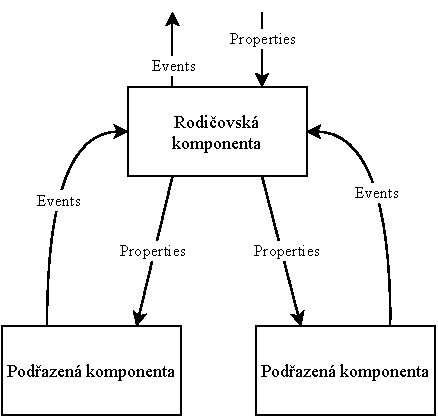
\includegraphics[width=0.75\textwidth]{media/vue.pdf}
    \caption{Doporučený způsob komunikace mezi komponentami ve Vue frameworku}
\end{figure}

\chapter{Požadavky na systém}
\textit{Tato kapitola shrnuje původní a později přidané požadavky na systém a jeho základní funkcionalitu.}

Cílem bylo vyrobit webovou aplikaci jež by uměla procházet data v RDF databázích podle předem navolenýcyh konfiguracích. Procházením se myslí postupné objevování nových uzlů grafu s pomocí již existujících.

\section{Konfigurace}
Konfigurací se rozumí uzel v RDF grafu který popisuje, jak by měla aplikace procházet datasety. Aktuálně může mít konfigurace tyto vlastnosti:

\begin{itemize}
    \item \texttt{dct:title} Název konfigurace \textit{(je možné zadat ve více jazycích)}
    \item \texttt{dct:description} Širší popis, čeho je možné s konfigurací dosáhnout \textit{(je možné zadat ve více jazycích)}
    \item \texttt{browser:hasVisualStyleSheet} Určuje, jak mají uzly v aplikaci vypadat. \textit{(popsáno dále)}
    \item \texttt{browser:startingNode} Doporučený uzel nebo uzly, kde začít s procházením grafu.
    \item \texttt{browser:resourceUriPattern} Regulární výraz popisující, jak by mělo vypadat IRI uzlu. Používá se v aplikaci jako nápověda uživateli, zda zadal správné IRI ještě než se pošle požadavek.
    \item \texttt{browser:hasViewSet} View sety. \textit{(popsáno dále)}
    \item \texttt{browser:autocomplete} JSON soubor se seznamem RDF uzlů podle kterých probíhá hledání. \textit{(popsáno dále)}
\end{itemize}

Příkladem konfigurace může být kupříkladu procházení slavných osobností na Wikidatech. Takováto konfigurace pak umožňuje uživateli chodit po uzlech reprezentující slavné osobnosti a dotazovat se například na filmy které natočily a knihy, které napsaly.

\section{ViewSet}
View set reprezentuje skupinu pohledů. Pravý smysl pohledů pochopí čtenář dále v textu. View set má následující vlastnosti:
\begin{itemize}
    \item \texttt{dct:title} Název view setu \textit{(je možné zadat ve více jazycích)}
    \item \texttt{browser:hasView} Pohledy které patří pod tento view set. \textit{(popsáno dále)}
    \item \texttt{browser:hasDefaultView} Výchozí pohled ze seznamu výše.
    \item \texttt{browser:hasCondition} todo
    \item \texttt{browser:hasDataset} todo
\end{itemize}

\section{View}
View (česky pohled) je způsob, jak můžeme pohlížet na konkrétní uzel v RDF grafu. Uzel totiž může mít obecně více vlastností současně, obdobně jako jedna osoba může být současně spisovatel, režisér a herec. V takovém případě bychom mohli mít tři různé pohledy na jeden uzel a uživatel si může vybírat, jestli ho zajímá jeho herecká, nebo spisovatelská kariéra. View má následující vlastnosti:

\begin{itemize}
    \item \texttt{dct:title} Název pohledu \textit{(je možné zadat ve více jazycích)}
    \item \texttt{dct:description} Popis pohledu \textit{(je možné zadat ve více jazycích)}
    \item \texttt{browser:hasExpansion} Odkaz na expanzi - určuje jaké uzly lze získat z daného uzlu \textit{(popsáno dále)}
    \item \texttt{browser:hasPreview} Odkaz na preview - určuje jaká data se mají získat pro ostylování konkrétního uzlu \textit{(popsáno dále)}
    \item \texttt{browser:hasDetail} Odkaz na detail - určuje která data se zobrazí v detailu konkrétního uzlu \textit{(popsáno dále)}
\end{itemize}

\section{Expansion}
Expansion popisuje jak lze daný uzel expandovat, tedy jedná se o operaci kdy se stahují nové uzly jež jsou nějak příbuzné expandovanému uzlu. Expanze vrací graf, tedy expandované uzly nemusí být přímými sousedy expandovaného. Jako expanzi si můžeme představit například \uv{Zobraz všechny knihy co napsala daná osoba}. Expanze formálně partří k pohledu (view).
\begin{itemize}
    \item \texttt{dct:title} Název expanze \textit{(je možné zadat ve více jazycích)}
    \item \texttt{browser:hasDataset} Popisuje kokrétní endpoint vůči kterému se dotazuje na data.
    \item \texttt{browser:query} Popisuje SPARQL dotaz který bude spuštěn na endpointu datasetu.
\end{itemize}
\citet[str.29]{Andel07}

\chapter*{Závěr}
\addcontentsline{toc}{chapter}{Závěr}


%%% Seznam použité literatury
%%% Seznam použité literatury (bibliografie)
%%%
%%% Pro vytváření bibliografie používáme bibTeX. Ten zpracovává
%%% citace v textu (např. makro \cite{...}) a vyhledává k nim literaturu
%%% v souboru literatura.bib.
%%%
%%% Příkaz \bibliographystyle určuje, jakým stylem budou citovány odkazy
%%% v textu. V závorce je název zvoleného souboru .bst. Styly plainnat
%%% a unsrt jsou standardní součástí latexových distribucí. Styl czplainnat
%%% je dodáván s touto šablonou a bibTeX ho hledá v aktuálním adresáři.

\bibliographystyle{czplainnat}    %% Autor (rok) s českými spojkami
% \bibliographystyle{plainnat}    %% Autor (rok) s anglickými spojkami
% \bibliographystyle{unsrt}       %% [číslo]

\renewcommand{\bibname}{Seznam použité literatury}

%%% Vytvoření seznamu literatury. Pozor, pokud jste necitovali ani jednu
%%% položku, seznam se automaticky vynechá.

\bibliography{literatura}

%%% Kdybyste chtěli bibliografii vytvářet ručně (bez bibTeXu), lze to udělat
%%% následovně. V takovém případě se řiďte normou ISO 690 a zvyklostmi v oboru.

% \begin{thebibliography}{99}
%
% \bibitem{lamport94}
%   {\sc Lamport,} Leslie.
%   \emph{\LaTeX: A Document Preparation System}.
%   2. vydání.
%   Massachusetts: Addison Wesley, 1994.
%   ISBN 0-201-52983-1.
%
% \end{thebibliography}


%%% Obrázky v bakalářské práci
%%% (pokud jich je malé množství, obvykle není třeba seznam uvádět)
\listoffigures

%%% Tabulky v bakalářské práci (opět nemusí být nutné uvádět)
%%% U matematických prací může být lepší přemístit seznam tabulek na začátek práce.
\listoftables

%%% Použité zkratky v bakalářské práci (opět nemusí být nutné uvádět)
%%% U matematických prací může být lepší přemístit seznam zkratek na začátek práce.
\chapwithtoc{Seznam použitých zkratek}

%%% Přílohy k bakalářské práci, existují-li. Každá příloha musí být alespoň jednou
%%% odkazována z vlastního textu práce. Přílohy se číslují.
%%%
%%% Do tištěné verze se spíše hodí přílohy, které lze číst a prohlížet (dodatečné
%%% tabulky a grafy, různé textové doplňky, ukázky výstupů z počítačových programů,
%%% apod.). Do elektronické verze se hodí přílohy, které budou spíše používány
%%% v elektronické podobě než čteny (zdrojové kódy programů, datové soubory,
%%% interaktivní grafy apod.). Elektronické přílohy se nahrávají do SISu a lze
%%% je také do práce vložit na CD/DVD. Povolené formáty souborů specifikuje
%%% opatření rektora č. 72/2017.
\appendix
\chapter{Přílohy}

\section{První příloha}

\openright
\end{document}
